\chapter{Song song hóa thuật toán giảm chiều (SVD)}

\section{Nhân ma trận}

Nhân ma trận là một phép toán nền tảng trong nhiều ứng dụng tính toán khoa học, mô phỏng số và học máy. Với hai ma trận  
\[
A \in \mathbb{R}^{m \times q}, \quad B \in \mathbb{R}^{q \times n},
\]  
ma trận kết quả \(C \in \mathbb{R}^{m \times n}\) được xác định bởi:
\[
c_{ij} = \sum_{k=1}^{q} a_{ik} b_{kj}.
\]
Thuật toán tuần tự thực hiện phép nhân ba vòng lặp lồng nhau với độ phức tạp \(O(n^{3})\). Điều này khiến việc thiết kế các thuật toán song song nhằm giảm thời gian thực thi trở thành một yêu cầu quan trọng trong các hệ thống tính toán hiệu năng cao (HPC).

\subsection{Phân chia dữ liệu}

Hiệu năng của một thuật toán song song phụ thuộc mạnh vào cách dữ liệu được phân phối lên các bộ xử lý. Ba phương pháp chính được xem xét trong luận văn này là phân chia một chiều (1D), hai chiều (2D) và ba chiều (3D). Mỗi phương pháp thể hiện mức độ cân bằng khác nhau giữa chi phí giao tiếp và khối lượng tính toán tại mỗi bộ xử lý.

\subsubsection{Phân chia một chiều (1D Partitioning)}

Trong phân chia 1D, ma trận \(A\) được chia theo hàng (hoặc cột) cho các bộ xử lý.  
Mỗi bộ xử lý giữ một phần của ma trận \(A\) và phải nhận toàn bộ ma trận \(B\) thông qua truyền thông.  

Phương pháp này đơn giản nhưng chi phí giao tiếp lớn, đặc biệt khi số bộ xử lý tăng cao. Thuật toán nhân ma trận theo mô hình 1D đạt độ phức tạp tính toán:
\[
T_{\text{comp}} = O\left( \frac{n^{3}}{p} \right),
\]
trong khi chi phí truyền thông có độ lớn:
\[
T_{\text{comm}} = O(n \log p).
\]

\subsubsection{Phân chia hai chiều (2D Block Partitioning)}

Trong phân chia 2D, ma trận \(A\) và \(B\) được chia thành các block kích thước đều nhau và phân phối lên lưới xử lý dạng \(p = q^{2}\).  
Mỗi bộ xử lý lưu một block của \(A\), \(B\) và tương ứng tạo ra một block của \(C\).  
Cách phân chia này giảm đáng kể lượng dữ liệu cần trao đổi, do mỗi bộ xử lý chỉ làm việc với block lân cận, nhờ đó mang lại hiệu năng tốt hơn so với phân chia 1D.

\subsubsection{Phân chia ba chiều (3D Partitioning)}

Phân chia 3D mở rộng cách tổ chức dữ liệu từ 2D sang cấu trúc khối ba chiều.  
Dữ liệu ma trận được nhân bản một phần theo chiều thứ ba, giúp giảm khối lượng tính toán tại mỗi bộ xử lý và đồng thời hạn chế xung đột giao tiếp.  
Đây là cơ sở của thuật toán DNS được trình bày ở phần sau.

\subsection{Thuật toán Broadcast 1D}

Thuật toán Broadcast 1D nhân ma trận dựa trên mô hình phân chia theo hàng. Mỗi bộ xử lý lưu một dải hàng của ma trận \(A\), trong khi ma trận \(B\) được broadcast tới tất cả các bộ xử lý.

Quy trình thực hiện gồm:
\begin{itemize}
    \item Chia các hàng của \(A\) cho các bộ xử lý.
    \item Broadcast toàn bộ ma trận \(B\).
    \item Mỗi bộ xử lý thực hiện phép nhân phần dữ liệu được giao.
\end{itemize}

Độ phức tạp song song của thuật toán:
\[
T(n,p) = O\left(\frac{n^{3}}{p} + n\log p \right),
\]
trong đó thành phần thứ hai thể hiện chi phí truyền thông của thao tác broadcast.

\subsection{Thuật toán Cannon}

Thuật toán Cannon triển khai trên lưới xử lý hai chiều.  
Dữ liệu ban đầu được căn chỉnh (skew) bằng cách dịch vòng các block của ma trận \(A\) theo hàng và các block của ma trận \(B\) theo cột. Sau quá trình căn chỉnh, thuật toán thực hiện \(q\) vòng lặp, mỗi vòng gồm:
\begin{itemize}
    \item Nhân block \(A_{ij}\) và \(B_{ij}\).
    \item Dịch block \(A\) sang trái một ô.
    \item Dịch block \(B\) lên trên một ô.
\end{itemize}

Thuật toán đạt:
\[
T_{\text{comp}} = O\left( \frac{n^{3}}{p} \right), \qquad
T_{\text{comm}} = O\left( \frac{n^{2}}{\sqrt{p}} \right),
\]
cho thấy mức độ cân bằng tốt giữa giao tiếp và tính toán, đặc biệt hiệu quả khi số bộ xử lý có thể sắp xếp thành lưới vuông.

\subsection{Thuật toán DNS (Dekel--Nassimi--Sahni)}

Thuật toán DNS sử dụng phân chia dữ liệu ba chiều, trong đó mỗi chiều tương ứng với một trong ba chỉ số \(i, j, k\) của phép nhân ma trận.  
Ma trận được ánh xạ vào một lưới khối lập phương các bộ xử lý, cho phép mỗi bộ xử lý chỉ thực hiện một phần rất nhỏ của phép nhân:

\[
A_{ik} \cdot B_{kj}.
\]

Dữ liệu được broadcast theo hai chiều và kết quả được reduce theo chiều còn lại để thu được phần tử tương ứng của ma trận \(C\).

Độ phức tạp song song:
\[
T(n,p) = O\left(\frac{n^{3}}{p^{3}} + \frac{n^{2}}{p^{2}}\log p + \log p\right).
\]

Mặc dù thuật toán mang lại hiệu năng lý thuyết rất cao, cấu trúc giao tiếp phức tạp và yêu cầu phân chia dữ liệu ba chiều khiến việc triển khai gặp nhiều thách thức trên các hệ thống thực tế.

\subsection{Đánh giá chung}

\begin{itemize}
    \item Phân chia 1D và thuật toán Broadcast phù hợp cho các hệ thống nhỏ hoặc bài toán không yêu cầu mở rộng mạnh.
    \item Phân chia 2D và thuật toán Cannon mang lại hiệu năng cao, cân bằng tốt giữa chi phí tính toán và truyền thông.
    \item Phân chia 3D và thuật toán DNS cung cấp hiệu năng lý thuyết tối ưu, song chi phí triển khai và đồng bộ dữ liệu lớn.
\end{itemize}

\section{Song song của biến thể phương pháp Jacobi cho ma trận đối xứng thực}

\begin{figure}[H]
\centering
\resizebox{0.60\textwidth}{!}{
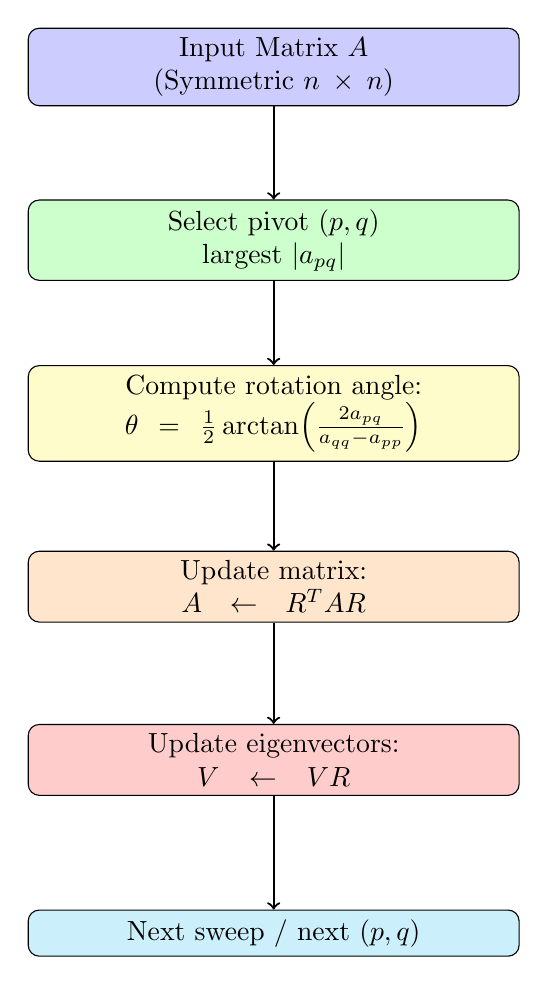
\begin{tikzpicture}[
    node distance=2.2cm,
    arrow/.style={->, thick},
    every node/.style={align=center}
]

% Nodes
\node (A) [rectangle, rounded corners, draw, fill=blue!20, text width=6cm] 
    {Input Matrix $A$\\(Symmetric $n\times n$)};

\node (select) [rectangle, rounded corners, draw, fill=green!20, text width=6cm, below of=A] 
    {Select pivot $(p,q)$\\largest $|a_{pq}|$};

\node (theta) [rectangle, rounded corners, draw, fill=yellow!20, text width=6cm, below of=select] 
    {Compute rotation angle:\\
    $\theta = \frac12 \arctan\!\left(\frac{2a_{pq}}{a_{qq}-a_{pp}}\right)$};

\node (updateA) [rectangle, rounded corners, draw, fill=orange!20, text width=6cm, below of=theta] 
    {Update matrix:\\
    $A \leftarrow R^T A R$};

\node (updateV) [rectangle, rounded corners, draw, fill=red!20, text width=6cm, below of=updateA] 
    {Update eigenvectors:\\
    $V \leftarrow V R$};

\node (loop) [rectangle, rounded corners, draw, fill=cyan!20, text width=6cm, below of=updateV] 
    {Next sweep / next $(p,q)$};

% Simple one-direction arrows
\draw [arrow] (A) -- (select);
\draw [arrow] (select) -- (theta);
\draw [arrow] (theta) -- (updateA);
\draw [arrow] (updateA) -- (updateV);
\draw [arrow] (updateV) -- (loop);

\end{tikzpicture}
}
\caption{Pipeline mô tả tính giá trị riêng vector riêng}
\end{figure}

\begin{algorithm}[H]
\caption{Thuật toán Song song Jacobi cho Ma trận Hiệp phương sai}
\label{alg:parallel_jacobi}
\begin{algorithmic}[1]
\Require Ma trận dữ liệu $X \in \mathbb{R}^{d \times d}$, ngưỡng hội tụ $\epsilon$, số vòng lặp tối đa $K_{max}$
\Ensure Ma trận giá trị riêng $\Lambda$, Ma trận vector riêng $V$

\State $V \leftarrow I_d$ \Comment{Khởi tạo ma trận đơn vị}
\State $idx \leftarrow [0, 1, \dots, d-1]$ \Comment{Khởi tạo mảng chỉ số}

\For{$k = 1$ \textbf{to} $K_{max}$}
    \State $converged \leftarrow \text{True}$
    
    \For{$step = 1$ \textbf{to} $d$} \Comment{Thực hiện một vòng quét (Sweep)}
        
        \State \textbf{Parallel Region:} \Comment{Phân chia công việc cho các luồng}
        \For{\textbf{each} pair $(p, q)$ generated from $idx$}
            
            \State \Call{Pivot}{$(p, q)$} \Comment{Xác định cặp phần tử cần khử}
            
            \If{$|X_{pq}| > \epsilon$}
                \State $converged \leftarrow \text{False}$
                \State $(c, s) \leftarrow$ \Call{COMPUTE\_ROTATION}{$X_{pp}, X_{qq}, X_{pq}$}
                \State \Call{UPDATE\_MATRX\_X}{$X, p, q, c, s$} \Comment{Cập nhật hàng/cột của X}
                \State \Call{UPDATE\_MATRIX\_V}{$V, p, q, c, s$} \Comment{Cập nhật cột của V}
            \EndIf
            
        \EndFor
        \State \textbf{End Parallel}
        
        \State \textbf{Barrier Synchronization} \Comment{Đồng bộ hóa các luồng}
        \State \Call{ROTATE\_INDICES}{$idx$} \Comment{Xoay vòng chỉ số Round-Robin}
        
    \EndFor

    \If{$converged$ is \text{True}}
        \State \textbf{break} \Comment{Thuật toán hội tụ}
    \EndIf
\EndFor

\State $\Lambda \leftarrow \text{diag}(X)$
\State \Return $\Lambda, V$

\end{algorithmic}
\end{algorithm}

Trong phạm vi bài toán này, dữ liệu đầu vào là ma trận thực $A \in \mathbb{R}^{m \times d}$. Mục tiêu là tính giá trị riêng và vector riêng của ma trận hiệp phương sai (hoặc ma trận Gram) $X = A^T A$.

Vì $X$ là ma trận đối xứng thực ($X = X^T$), nó thỏa mãn tính chất của ma trận chuẩn (normal matrix). Do đó, các phép biến đổi "Cắt" (Shear) và "Chéo" (Diagonal) trong phương pháp giảm chuẩn tổng quát của Eberlein trở nên không cần thiết (chúng trở thành các phép đồng nhất). Thuật toán lúc này quy về Phương pháp Jacobi cổ điển, chỉ sử dụng các phép quay trực giao để khử các phần tử ngoài đường chéo, nhưng được tổ chức theo chiến lược song song.

\subsection{Mục tiêu và giả thiết}
\begin{itemize}
    \item \textbf{Đầu vào:} Ma trận dữ liệu $A \in \mathbb{R}^{m \times d}$, từ đó tính $X = A^T A \in \mathbb{R}^{d \times d}$.
    \item \textbf{Mục tiêu:} Tìm ma trận trực giao $Q$ và ma trận đường chéo $\Lambda$ sao cho $Q^T X Q = \Lambda$. Các phần tử trên đường chéo của $\Lambda$ là các giá trị riêng, và các cột của $Q$ là các vector riêng tương ứng.
\end{itemize}

\subsection{Chiến lược song song hóa}
Để tận dụng kiến trúc đa xử lý, thuật toán không chọn phần tử lớn nhất để khử (như phương pháp cổ điển tuần tự) mà sử dụng chiến lược chia cặp và xoay vòng:

\begin{itemize}
    \item \textbf{Chiến lược chia cặp (Pairing Strategy):} Tại mỗi bước, $d$ hàng/cột của ma trận $X$ được chia thành $d/2$ cặp chỉ số $(p, q)$ rời nhau. Điều này cho phép $d/2$ luồng tính toán thực hiện khử đồng thời các phần tử $X_{pq}$ mà không tranh chấp dữ liệu.
    
    \item \textbf{Xoay vòng chỉ số (Round-Robin):} Sau mỗi bước tính toán, các chỉ số được hoán vị theo quy tắc Round-Robin (giữ nguyên chỉ số đầu, dịch vòng tròn các chỉ số còn lại). Một chu kỳ đầy đủ (sweep) gồm $d-1$ bước (với $d$ chẵn) đảm bảo mọi cặp phần tử ngoài đường chéo đều được xử lý ít nhất một lần.
\end{itemize}

\subsection{Quy trình tính toán tại mỗi bước}
Tại mỗi bước $k$, với mỗi cặp $(p, q)$ được phân công cho một luồng xử lý, các thao tác sau được thực hiện:

\paragraph{Tính tham số quay}
Mục tiêu là tìm phép quay Jacobi $J_{p,q}$ để triệt tiêu phần tử $X_{pq}$. Các tham số $\tau, t, c, s$ được tính như sau:
\[
\tau = \frac{X_{qq} - X_{pp}}{2 X_{pq}}
\]
\[
t = \frac{\operatorname{sgn}(\tau)}{|\tau| + \sqrt{1+\tau^2}}
\]
\[
c = \frac{1}{\sqrt{1+t^2}}, \qquad s = t \cdot c
\]
Trong đó $c = \cos\theta$ và $s = \sin\theta$.

\paragraph{Cập nhật ma trận $X$}
Áp dụng phép biến đổi tương đồng $X^{(k+1)} = J_{p,q}^T X^{(k)} J_{p,q}$.
\begin{itemize}
    \item \textbf{Cập nhật phần tử đường chéo ($p, q$):}
    \[
    \begin{aligned}
    X'_{pp} &= c^2 X_{pp} + s^2 X_{qq} - 2cs\, X_{pq} \\
    X'_{qq} &= s^2 X_{pp} + c^2 X_{qq} + 2cs\, X_{pq} \\
    X'_{pq} &= X'_{qp} = 0 \quad (\text{Gán cứng để tránh sai số})
    \end{aligned}
    \]
    \item \textbf{Cập nhật phần tử ngoài đường chéo ($j \neq p, q$):}
    Các hàng và cột liên quan đến $p$ và $q$ được cập nhật song song:
    \[
    \begin{aligned}
    X'_{pj} &= c\, X_{pj} - s\, X_{qj} \\
    X'_{qj} &= s\, X_{pj} + c\, X_{qj}
    \end{aligned}
    \]
    Do tính đối xứng, ta cập nhật đồng thời: $X'_{jp} = X'_{pj}$ và $X'_{jq} = X'_{qj}$.
\end{itemize}

\paragraph{Cập nhật ma trận vector riêng $V$}
Ma trận $V$ (khởi tạo là ma trận đơn vị $I$) tích lũy các phép quay để tạo thành ma trận vector riêng cuối cùng:
\[
\begin{aligned}
V'_{:,p} &= c\, V_{:,p} - s\, V_{:,q} \\
V'_{:,q} &= s\, V_{:,p} + c\, V_{:,q}
\end{aligned}
\]

\subsection{Nhận xét}
Biến thể này kết hợp được ưu điểm về tốc độ hội tụ bậc hai của phương pháp Jacobi cổ điển trên ma trận đối xứng với khả năng mở rộng hiệu năng của chiến lược song song. Việc loại bỏ các phép biến đổi phức tạp (Shear) giúp giảm đáng kể chi phí tính toán trên mỗi bước lặp so với thuật toán Norm-Reducing tổng quát.


\section{Song song hóa các phần còn lại}
\subsection{Song song hóa tính giá trị kì dị}

Sau khi tính được ma trận \(\Lambda\) chứa \(d\) giá trị riêng, bước tiếp theo là xác định \(d\) giá trị kì dị tương ứng. Để tận dụng khả năng tính toán song song, chúng ta chia tổng số phép toán cho mỗi luồng (thread) như sau:

\[
\text{số phép toán mỗi luồng} = \frac{d}{p},
\]

trong đó \(p\) là số lượng luồng được sử dụng. Mỗi luồng sẽ chịu trách nhiệm tính giá trị kì dị của một tập con các giá trị riêng, đảm bảo rằng tất cả các giá trị kì dị được tính toán đồng thời và độc lập, từ đó tăng tốc độ tính toán tổng thể. vậy độ phức tạp thuật toán của phần này là $T_{1} = o(\frac{n}{p})$.

\subsection{Song song hóa sắp xếp theo giá trị kì dị}

Giả sử chúng ta có \(k\) giá trị riêng và các vector riêng tương ứng. Để sắp xếp các giá trị kì dị theo thứ tự giảm dần (hoặc tăng dần) và đồng thời sắp xếp lại các cột của ma trận vector riêng, chúng ta áp dụng song song hóa như sau:

\begin{itemize}
    \item Chia dữ liệu luồng: Mỗi luồng nhận một tập con các cặp giá trị riêng, vector riêng cần sắp xếp. Nếu có \(p\) luồng, mỗi luồng xử lý khoảng \(\frac{k}{p}\) cặp.  
    \item Sắp xếp trong luồng: Mỗi luồng sắp xếp các giá trị kì dị của nó độc lập, đồng thời sắp xếp các vector riêng tương ứng.  
    \item Gộp kết quả: Sau khi tất cả luồng hoàn tất, các kết quả được merge để thu được thứ tự cuối cùng. Merge có thể thực hiện theo kiểu merge-sort song song, đảm bảo kết quả chính xác.  
\end{itemize}
Do vậy, tổng số phép toán của thuật toán song song có thể ước lượng là:
\[
T_2 = O\Big(\frac{n}{p} \log(n) - \log(p) + np\Big),
\]
trong đó \(n\) là số phần tử (giá trị kì dị) và \(p\) là số lượng luồng.

\subsection{Chuyển vị ma trận}
Để tăng hiệu quả tính toán, Ấp dụng phương pháp blocked parallel transpose kết hợp với OpenMP. Cụ thể, ma trận $A \in \mathbb{R}^{m \times n}$ được chia thành các block kích thước $B \times B$, và mỗi block được xử lý độc lập bởi một luồng:

\[\begin{matrix}
B[jj][ii] &=& A[ii][jj], \\
ii&=&i,\dots,\min(i+B-1,M-1), \\ jj&=&j,\dots,\min(j+B-1,N-1),
\end{matrix}\]

trong đó $(i,j)$ là tọa độ bắt đầu của block và $B$ là kích thước block.  

Các block được phân phối cho $p$ luồng sử dụng chỉ thị OpenMP với `collapse(2)` để song song hóa cả hai vòng lặp bên ngoài. Kỹ thuật này vừa tận dụng tối đa khả năng đa luồng, vừa giảm thiểu cache-miss nhờ truy cập dữ liệu liên tiếp trong mỗi block.  

Cách tiếp cận này đảm bảo rằng các phép toán transpose trên từng block là độc lập, tránh hiện tượng race condition, đồng thời cung cấp tốc độ tính toán cao khi làm việc với ma trận lớn.
